\documentclass{zirkelblatt1415}

\usepackage[bottom=4cm]{geometry}

\usepackage{textcomp}

\newcommand{\RR}{\mathbb{R}}
\newcommand{\CC}{\mathbb{C}}
\newcommand{\ZZ}{\mathbb{Z}}
\renewcommand{\NN}{\mathbb{N}}
\newcommand{\QQ}{\mathbb{Q}}
%\newcommand{\K}{\mathbb{K}}
\newcommand{\PP}{\mathbb{P}}
%\newcommand{\CP}{\mathbb{CP}}
%\newcommand{\RP}{\mathbb{RP}}
\newcommand {\kk} {\Bbbk}
\newcommand{\VV}{\mathbb V}
\newcommand{\HH}{\mathbb{H}}
\newcommand{\ii}{\mathrm{i}}

\renewcommand{\Re}{\operatorname{Re}}
\renewcommand{\Im}{\operatorname{Im}}

\newcommand{\lra}{\longrightarrow}
\newcommand{\ol}[1]{\overline{#1}}

%\setlength{\parindent}{0cm}
%\usepackage{tikz}
\usepackage{tkz-euclide}
\usetkzobj{all}

%\usetikzlibrary{arrows,calc}
%\tikzset{
%Define standard arrow tip
%>=stealth',
%Define style for different line styles
%help lines/.style={dashed, thick},
%axis/.style={<->},
%important line/.style={thick},
%connection/.style={thick, dotted},
%}

\begin{document}

\maketitle{Komplexe Zahlen}{Erster}

\tableofcontents

\section{Zahlenbereiche}

In diesem Brief soll es um Zahlen gehen. Das klingt langweilig? Nicht doch! Im Laufe eures Lebens seid ihr schon vielen verschiedenen Zahlen begegnet: Als kleine Kinder konntet ihr nur zählen, d.\,h. ihr kanntet nur die \emph{nat\"urlichen Zahlen} 1, 2, 3, \ldots Viele Jahre lang waren diese auch v\"ollig ausreichend und ihr habt in der Grundschule gelernt, damit zu rechnen, so gut es halt ging: Addieren und Multiplizieren war problemlos m\"oglich, Subtrahieren und Dividieren aber nur mit Einschr\"ankungen.

In der f\"unften Klasse lerntet %die form hab ich extra im Duden nachgeschaut!
ihr die negativen Zahlen kennen, die zusammen mit den natürlichen Zahlen die \emph{ganzen Zahlen} bilden. Ein weiteres Jahr sp\"ater kamen Br\"uche und damit die \emph{rationalen Zahlen}. Diese bilden zusammen mit den irrationalen Zahlen wie beispielsweise die Kreiszahl $\pi=3{,}1415926\ldots$ die \emph{reellen Zahlen}.

Bei jeder neuen Erweiterung fanden die Menschen die \glqq neuen\grqq\ Zahlen als v\"ollig unn\"otig und trotzdem verwenden wir sie heute, als w\"aren sie das Selbstverst\"andlichste der Welt. Wir wollen in diesem Brief mit euch \emph{noch mehr} Zahlen kennen lernen. Ihr glaubt, dass das nicht geht und die reellen Zahlen ja schon alles sind? Dann lasst euch \"uberraschen!
\medskip \\
Wir beginnen mit einer kurzen \"Ubersicht \"uber alle Zahlbereiche, die ihr schon kennt, und erkl\"aren, wof\"ur Menschen diese Zahlbereiche einf\"uhrten und bis wann sie von diesen Zahlbereichen noch \"uberhaupt nichts wussten.

\subsection{Natürliche Zahlen}

\emph{Definition:} $\NN=\{0,1,2,3,4,\ldots\}$

\emph{Erfunden, um} Objekte zu zählen.

\emph{Intuitive Bedeutung:} \emph{Anhäufen, Verschieben} oder \emph{Zählen}

\emph{Merkwürdig bis} ca. 1500 v.\,Chr. Die Null wurde wohl als eigenständige Zahl von den Indern um 500 n.\,Chr. das erste Mal benutzt, wurde aber erst in Inden um 900 n.\,Chr. und in Europa im 12. Jahrhundert regelmäßig verwendet.

%-------------------------------------------------------------

\subsection{Ganze Zahlen}

\emph{Definition:} $\ZZ=\{\ldots,-3,-2,-1,0,1,2,3,\ldots\}$

\emph{Erfunden, um} mit "`Schulden"' einfach Rechnen zu können. Zum Beispiel, was ist $3-5$? Oder wenn ich dir zwei Goldtaler gebe, du mir drei zurückgibst, wieviel schulde ich dir?

\emph{Intuitive Bedeutung} der negativen Zahlen: \emph{Gegenteil von Besitz, Schuld} oder \emph{Gegenrichtung}. Anstatt zu vermehren wird etwas \emph{vermindert}.

\emph{Merkwürdig bis} zum 17. Jahrhundert in Europa. Erste Erwähnungen aber bereits 200 vor bis 200 nach Christus in China.

%-------------------------------------------------------------

\subsection{Rationale Zahlen}

\emph{Definition:} $\QQ=\left\{0,1,-1,\frac{1}{2},-\frac{1}{2},2,-2,\frac{1}{3},\frac{2}{3},-\frac{1}{3},\frac{2}{3},\ldots\right\}$, also alle Zahlen, die sich als Bruch von zwei ganzen Zahlen schreiben lassen.

\emph{Erfunden, um} Verhältnisse beschreiben zu können sowie Fragen \'a la \glqq Welche Zahl mit Drei multipliziert ist gleich Zwei?\grqq\ beantworten zu können.

\emph{Intuitive Bedeutung} von Brüchen sind Verhältnisse.

\emph{Merkwürdig bis} ca. 300 v.\,Chr. Benutzt und intuitiv als Verhältnis verstanden wurden sie bereits von den Indern, Ägyptern und Griechen.

\emph{Rechenregeln} Rationale Zahlen können addiert, subtrahiert, multipliziert und dividiert werden (außer durch Null!). Wichtig dafür ist, dass man Brüche \emph{erweitern} kann, wie in
\begin{equation*}
  \frac{2}{3}=\frac{2\cdot 4}{3\cdot 4}=\frac{8}{12}.
\end{equation*}

\begin{aufgabe}{Rechnen mit rationalen Zahlen (zum Aufwärmen)}
  \begin{enumerate}
    %\item Mache dir klar, dass \emph{Erweitern} eines Bruchs wie oben die gleiche Zahl beschreibt.
    \item Angenommen, zwei rationale Zahlen haben den gleichen \emph{Nenner}, also die natürliche Zahl unter dem Bruchstrich. Was bedeutet ihre Summe anschaulich? Wie kann man diese berechnen?
		\item Was ist $\frac{3}{7}+\frac{2}{5}$? Was ist $\frac{3}{7}-\frac{3}{5}$?
    \item Was bedeutet die Multiplation von zwei rationalen Zahlen anschaulich?
		\item Wie kann man das Produkt von zwei rationalen Zahlen berechnen? Was ist $\frac{3}{4}\cdot\frac{12}{9}$?
  \end{enumerate}
\end{aufgabe}

% \loesung{4cm}

% \newpage

\begin{aufgabe}{Inverse von rationalen Zahlen}
Das \emph{Inverse} einer Zahl ist diejenige Zahl, welche mit der gegebenen Zahl mutlipliziert gleich Eins ist. 
\begin{enumerate}
  \item Wie kann man das Inverse einer rationalen Zahl $\frac{a}{b}$ berechnen? Was ist das Inverse von $\frac{2}{3}$?  
  \item Division ist nichts anderes als das Multiplizieren mit dem Inversen einer Zahl. Was ist $\frac{2}{5}:\frac{4}{5}$? Was bedeutet das anschaulich?
\end{enumerate}
\end{aufgabe}

% \loesung{4cm}


%-------------------------------------------------------------

\subsection{Reelle Zahlen}

\emph{Definition:} $\RR=\{0{,}323454,\ 0,\ 5,\ 0{,}33\ol{33},\ -17,\ -3{,}14125868,\ \ldots\}$, das heißt alle Zahlen, die sich als "`unendliche Kommazahlen"' %hier stand vorher Dezimalbruch, aber eine kurze Googlesuche ergab bei mir, dass das nur *endliche* Kommazahlen sind, also alle Zahlen, die sich als Bruch mit einer Zehnerpotenz im Nenner schreiben lassen.
schreiben lassen. Dabei muss die Dezimaldarstellung nicht irgendwann aufhören, es sind unendliche sich-nicht-wiederholende Ausdrücke erlaubt. Die ganzen Zahlen sind in den reellen enthalten (man schreibt $\ZZ\subset\RR$) und die rationalen genauso, $\QQ\subset\RR$. Dies liegt daran, dass Brüche immer geschrieben werden können als endliche Dezimalzahlen oder unendliche sich wiederholende (sogenannte \emph{periodische}) Dezimalzahlen.

\emph{Erfunden, um} die Frage zu beantworten, welche Zahl mit sich selbst multipliziert gleich~$2$ ist.

\emph{Intuitive Bedeutung} der irrationalen Zahlen: als "`Grenzwerte"' von rationalen Zahlen und Lösungen von Gleichungen, in denen Zahlen mit sich selbst multipliziert werden.

\emph{Merkwürdig bis} ca. 1000 n.\,Chr. Entdeckt wurden die irrationalen Zahlen bereits ca. 500 v.\,Chr. von den Pythagoräern und sind auch in Euklids \emph{Elemente\footnote{Euklid hat ca. 300 v.\,Chr. alles mathematische Wissen seiner Zeit in den 13 B\"uchern mit dem Titel \glqq Die Elemente\grqq\ aufgeschrieben.}} vermerkt.

\emph{Beispiele:} $\pi=3{,}1415926535\ldots$, $e=2{,}718281828459045235360287471352662\ldots$ oder $\sqrt{2}=1{,}414213562373095048801688724209698078569671875376948073176\ldots$


\begin{aufgabe}{Irrationalität der Quadratwurzel aus Zwei}
Die \emph{Quadratwurzel aus Zwei} ist diejenige positive Zahl, die mit sich selbst multipliziert Zwei ergibt: $x \cdot x = 2$.
In dieser Aufgabe beweist du, dass die Quadratwurzel aus Zwei keine rationale
Zahl sein kann und daher irrational ist. Das ist ein ganz erstaunliches Resultat, das manche als die Geburtsstunde der Mathematik sehen: Ob wir es wollen oder nicht -- es gibt sehr anschauliche Zahlen, die nicht rational sind.
\begin{enumerate}
   \item Nimm einfach das Gegenteil an, nämlich, dass $x$ rational ist. Wie lässt sich dann $x$ laut der Definition von rationalen Zahlen schreiben?
   \item Angenommen es gilt jetzt $2\cdot a\cdot a=b\cdot b$ wobei $a$ und $b$ natürliche Zahlen sind und gekürzt wurden, also ihr größter gemeinsamer Teiler gleich Eins ist. Zeige, dass dann $b$ durch $2$ teilbar ist.
   \item Folgere analog, dass $a$ durch $2$ teilbar ist.
   \item Warum ist das ein Widerspruch und warum folgt daraus, dass $x$ irrational ist?
 \end{enumerate}
\end{aufgabe}

\begin{aufgabe}{Die Quadratwurzel aus Zwei anschaulich}
Die Quadratwurzel aus Zwei ist keine besonders seltsame Zahl. Wenn du den
\emph{Satz von Pythagoras} schon kennst, dann beweise folgendes: Die Länge der Diagonalen in einem Quadrat mit Seitenlänge Eins ist die Quadratwurzel aus Zwei.
\end{aufgabe}

% \newpage

% \loesung{5cm}

\section{Komplexe Zahlen}

\subsection{Motivation und Definition}

Was für Gleichungen können wir mit den rellen Zahlen lösen? Beispiele sind $x+5=2$, $3x=2$ und $x\cdot x=2$, wobei wir für jede Gleichung davon einen neuen Zahlenbereich einführen mussten: F\"ur $x+5=2$ die negativen Zahlen, f\"ur $3x=2$ die rationalen Zahlen und f\"ur $x\cdot x=2$ die reellen Zahlen. Welche anderen Gleichungen gibt es noch? Die vielleicht interessanteste Frage ist:
\begin{center}
Welche Zahl ergibt mit sich selbst multipliziert minus Eins?
\end{center}
In Gleichungen bedeutet dies: Welche Zahl $x$ erf\"ullt $x\cdot x=-1$? Wenn $x=1$ wäre, hätten wir $x^2=x\cdot x=1 \cdot 1 =1$. Wäre $x=-1$, dann hätten wir $x^2=(-1)\cdot(-1)=1$. Auch wenn wir jede andere relle Zahl mit sich selber multiplizieren, ist das Ergebnis immer positiv. Daher gibt es keine reelle Zahl, die $x^2=-1$ löst.


\textbf{Definition.} Deswegen definieren wir einfach eine neue Zahl, die diese Gleichung löst und nennen sie $\ii$, die imaginäre Einheit. Sie erfüllt demnach $\ii^2=-1$. Wir wollen außerdem, dass alle bisherigen Rechenregeln weiter gelten, wir können $\ii$ beim Rechnen also wie eine reelle Zahl behandeln, nur dass sie eben $\ii^2=-1$ erfüllt.\footnote{Die imaginäre Einheit~$\ii$ hat sich um 1600 einigen Mathematikern regelrecht aufgedrängt. Man kannte nämlich schon eine bestimmte Formel zum Lösen von kubischen Gleichungen. Die war umgemein praktisch und hat in vielen Fällen auch wunderbar funktioniert -- aber leider nicht immer. In manchen Fällen muss man bei dieser Formel nämlich Zahlen verwenden, deren Quadrat negativ ist. Das gelingt nur unter Verwendung der imaginären Einheit.}

\subsection{Geometrische Vorstellung}

Die gewohnten Rechenoperationen kann man sich alle auch geometrisch vorstellen. Wenn wir zum Beispiel eine Zahl mit $-1$ multiplizieren, bedeutet das auf dem Zahlenstrahl, dass wir diese Zahl an der Null spiegeln.

Das Multiplizieren mit einer positiven reellen Zahl entspricht dem Strecken des Abstands von der Null.

Was entspricht aber nun der Multiplikation mit $\ii$?

\newpage

\begin{aufgabe}{Was macht $\ii$?}
\begin{enumerate}
  \item Zeichne eine Zahlengerade sowie die Strecke von $0$ bis $1$, diese soll zur Zahl $1$ gehören. Welcher Strecke entspricht die Zahl $-1$? Was ist mit der $4$, der $-\frac{1}{2}?$
% \item Was bedeutet die Gleichung $1\cdot x\cdot x=-1$ geometrisch, wenn wir $x$ als \glqq geometrische Operation\grqq\ auffassen? Damit ist folgendes gemeint: 
  \item Nimm irgendeine Zahl auf dem Zahlenstrahl, zum Beispiel deine Lieblingszahl. Multipliziere diese Zahl mit~$\ii$. Momentan können wir uns noch nicht vorstellen, was das Ergebnis geometrisch sein soll. Lass dich davon aber nicht beirren, und multipliziere das Ergebnis ein zweites Mal mit~$\ii$. Wenn du die Rechenregel~$\ii \cdot \ii = -1$ verwendest, kannst du ganz klar sagen, welche Zahl hier herauskommt.
  \item Wenn du Teilaufgabe~b) verstanden hast, weißt du also folgendes: Wenn man eine Zahl \emph{zweimal} mit~$\ii$ multipliziert, kommt das auf dasselbe heraus, wie wenn man die Zahl an der Null spiegelt. Das \emph{einmalige Multiplizieren} mit~$\ii$ muss also irgendeine kuriose Operation sein, die, wenn man sie \emph{zweimal} ausführt, dasselbe macht wie Spiegelung an der Null.

Welche geometrischen Operationen (Strecken, Zerren, Spiegeln, Drehen, \ldots) kennst du, die ebenfalls diese Eigenschaft haben?
\end{enumerate}
\end{aufgabe}

Aus der vorherigen Aufgabe sieht man, dass wir nun eine Zahlenebene anstatt einer Zahlengeraden betrachten sollten. Die Ebene nennt man dann auch \emph{Gaußsche Zahlenebene}. Die Zahl $\ii$ liegt in dieser Ebene auf der $y$-Achse in Abstand $1$ vom Ursprung und hat dementsprechend $(x,y)$-Koordinaten $(0,1)$ (siehe Grafik links). Wie dort angedeutet entspricht die Multiplikation mit $\ii$ der Drehung um $90^{\textdegree}$ gegen den Uhrzeigersinn. Die Zahl $3\cdot\ii$ liegt bei den Koordinaten $(0,3)$, in der Grafik also oberhalb des Ausschnitts. Auch hier sieht man, dass wenn man die Zahl $3$ mit $\ii$ multipliziert, diese anschaulich um $90^{\textdegree}$ gedreht wird.

Es gibt noch eine zweite Drehung, die zweimal hintereinander ausgeführt die Spiegelung am Ursprung ergibt, diese ist auf der rechten Grafik eingezeichnet. Die Drehung um $270^{\textdegree}$ gegen den Uhrzeigersinn entspricht der Zahl $-\ii$.


\begin{minipage}{0.5\textwidth}
\centering
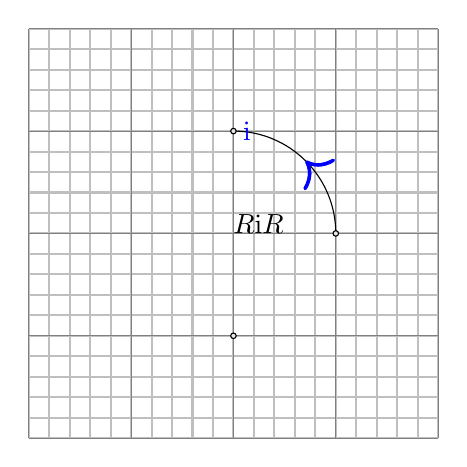
\begin{tikzpicture}[scale=1.3, decoration={markings, mark=at position 0.5 with {\arrow[scale=3, blue]{>}};}]
  \tkzInit[xmax=2,ymax=2,xmin=-2,ymin=-2]
   %\draw[ thick,latex-latex] (-1,4) -- (4,-6) node[anchor=south west] {$a$}; % two points for drawing 2x+y=2
  %\tkzText[above](0,6.75){Desired Output}
   \tkzDefPoint(0,0){O}
   \tkzDefPoint(1,0){Eins}
   \tkzDefPoint(0,1){IE}
   \tkzDefPoint(0,-1){mIE}
   \tkzDrawSegments(O,Eins O,IE O,mIE)
   \tkzGrid[sub]
   \tkzMarkAngle[fill=blue!25, size=1, postaction={decorate}](Eins,O,IE)
   %\tkzMarkAngle[fill=blue!25,mkpos=.2, size=1, decoration={markings, mark=at position 1 with {\arrow[scale=4,blue]{>}}}, postaction={decorate}](Eins,O,IE)
   %\tkzMarkAngle[fill=red!25,mkpos=.2, size=0.4](Eins,O,mIE)
   \tkzDrawPoints(Eins, IE, mIE)
   %\tkzLabelPoint[above right](Eins){$1$}
   \tkzLabelPoint[right](IE){\textcolor{blue}{$\ii$}}
   %\tkzLabelPoint[right](mIE){\textcolor{red}{$-\ii$}}
   \tkzAxeX[label=$\RR$, orig=false]
   \tkzAxeY[label=$\ii\RR$]
\end{tikzpicture}
\end{minipage}
\begin{minipage}{0.5\textwidth}
\centering
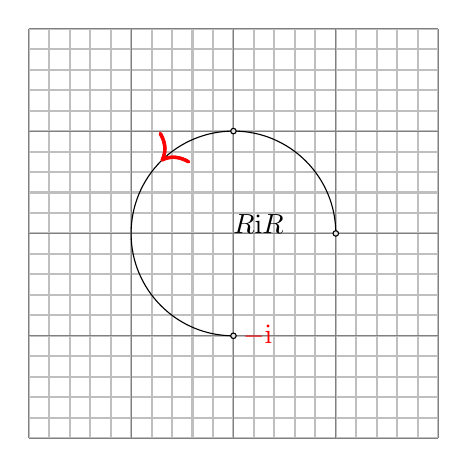
\begin{tikzpicture}[scale=1.3, decoration={markings, mark=at position 0.5 with {\arrow[scale=3, red]{>}};}]
  \tkzInit[xmax=2,ymax=2,xmin=-2,ymin=-2]
   %\draw[ thick,latex-latex] (-1,4) -- (4,-6) node[anchor=south west] {$a$}; % two points for drawing 2x+y=2
  %\tkzText[above](0,6.75){Desired Output}
   \tkzDefPoint(0,0){O}
   \tkzDefPoint(1,0){Eins}
   \tkzDefPoint(0,1){IE}
   \tkzDefPoint(0,-1){mIE}
   \tkzDrawSegments(O,Eins O,IE O,mIE)
   \tkzGrid[sub]
   %\tkzMarkAngle[fill=blue!25,mkpos=.2, size=0.4](Eins,O,IE)
   \tkzMarkAngle[fill=red!25, size=1, postaction={decorate}](Eins,O,mIE)
   \tkzDrawPoints(Eins, IE, mIE)
   %\tkzLabelPoint[above right](Eins){$1$}
   %\tkzLabelPoint[right](IE){\textcolor{blue}{$\ii$}}
   \tkzLabelPoint[right](mIE){\textcolor{red}{$-\ii$}}
   \tkzAxeX[label=$\RR$, orig=false]
   \tkzAxeY[label=$\ii\RR$]
\end{tikzpicture}
\end{minipage}


Was ist $1+\ii$? Mit Sicherheit keine reelle Zahl! Kann $1+\ii=\ii$ gelten? Was ginge schief dabei?
\begin{aufgabe}{Eine falsche Gleichung}
Noch wissen wir nicht besonders viel über~$\ii$. Aber trotzdem können wir schon
verstehen, dass die Gleichung~$1 + \ii = \ii$ nicht gelten kann. Wieso nicht?
\end{aufgabe}

Also muss $1+\ii$ tats\"achlich eine neue Zahl sein und wir k\"onnen auch alle Summen aus reellen und imagin\"aren Zahlen betrachten. Das sind \emph{komplexe Zahlen}. Zahlen wie $\ii$ (statt beispielsweise $1+\ii$) haben aber auch  noch einen besonderen Namen: Eine \emph{rein imaginäre Zahl} ist ein Produkt einer reellen Zahl und $\ii$, also zum Beispiel $\ii$, $3\ii$ oder auch $\pi\ii$.

\textbf{Definition.} Die Menge der \emph{komplexen Zahlen} ist die Menge aller Summen einer reellen Zahl und einer rellen Zahl multipliziert mit $\ii$. In Formeln also
\begin{equation*}
  \CC=\{a+\ii b, \text{ wobei $a$ und $b$ beliebige reelle Zahlen sind}\}.
\end{equation*}
Beispiele für komplexe Zahlen sind: $3 + 5\ii$, $100 - 21\ii$, $5\ii$ (das ist dasselbe wie $0+5\ii$). Auch die gewöhnlichen reellen Zahlen zählen als komplexe Zahlen (also ist zum Beispiel~$42$ eine komplexe Zahl). Das ist ganz genauso wie bei den anderen Zahlenbereichen: Jede natürliche Zahl ist auch eine ganze Zahl und jede ganze Zahl ist auch eine rationale.

Wie bereits vorher erwähnt sollen für die komplexen Zahlen die üblichen Rechenregeln gelten, also zum Beispiel das Distributivgesetz, so dass
\[ a+\ii b+\ii c=a+\ii(b+c), \]
wobei $a,b,c\in\RR$ sind. Außerdem gilt $\ii+0=\ii=\ii\cdot 1$ und $0\cdot\ii =0$.

\begin{aufgabe}{Gauß und seine Zahlenebene}
Die horizontale Achse in der Gaußschen Zahlenebene soll die Zahlengerade der reellen Zahlen sein, also derjenigen komplexen Zahlen $x=a+\ii b$ mit $b=0$. Die vertikale Achse soll die rein imagin\"aren Zahlen $x=a+\ii b$ mit $a=0$ beschreiben. Zeichne die folgenden Zahlen in die komplexe Zahlenebene: $1$, $\ii$, $1+\ii$, $\frac{1+\ii}{2}$, $-\ii$, $4-2\ii$ und $\frac{30}{8}\ii$.
\end{aufgabe}

\begin{center}
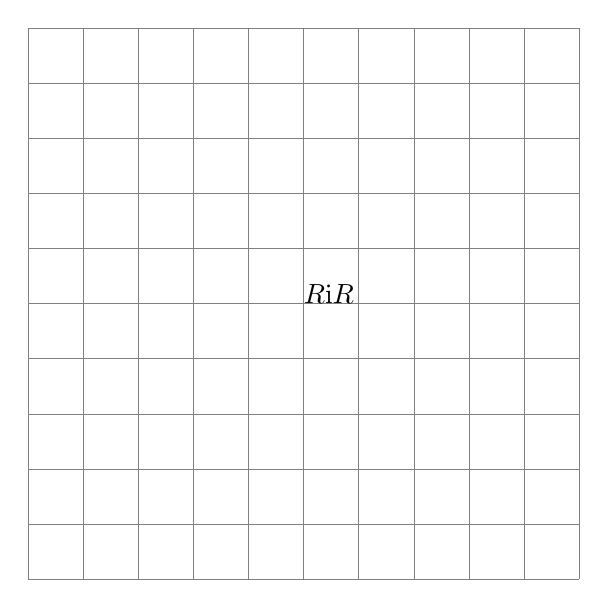
\begin{tikzpicture}[scale=0.7]
  \tkzInit[xmax=5,ymax=5,xmin=-5,ymin=-5]
   \tkzGrid
   \tkzAxeX[label=$\RR$]
   \tkzAxeY[label=$\ii\RR$]
   %\draw[ thick,latex-latex] (-1,4) -- (4,-6) node[anchor=south west] {$a$}; % two points for drawing 2x+y=2
  %\tkzText[above](0,6.75){Desired Output}
\end{tikzpicture}
\end{center}

\subsection{Grundrechenarten}

Schauen wir uns mal ein paar Beispiele für Rechnungen mit den komplexen Zahlen an:
\begin{align*}
  -2+\ii+17\ii+2&=18\ii \\
  \ii\cdot(1+\ii)&=\ii+\ii^2=\ii-1=-1+\ii\\
  (3-4\ii)\cdot(7+\ii)&=21-28\ii+3\ii-4\ii^2=21+(-28+3)\ii-4\cdot(-1)=25-25\ii\\
\end{align*}

\begin{aufgabe}{Ein paar Rechnungen}
  Vereinfache die folgenden komplexen Zahlen soweit wie möglich:
  \begin{align*}
    \ii+6-2\ii&= \hspace{10cm}\\[0.4em]
    (2\ii-3)\cdot(1+\ii)&= \\[0.4em]
    \frac{1}{\ii}&=
  \end{align*}
\end{aufgabe}
Die letzte Aufgabe wirft die Frage auf, wie man eigentlich Inverse von komplexen Zahlen berechnet, d.\,h. wie man durch komplexe Zahlen dividiert. Dies k\"onnen wir nach dem n\"achsten Abschnitt ausf\"uhrlicher behandeln.

\subsection{Konjugation und Imaginär- sowie Realteil}

\textbf{Definition.} Gegeben sei eine komplexe Zahl $z\in\CC$ mit $z=a+\ii b$ mit $a,b\in \RR$. Dann hei\ss t $\Re(z)=a$ der \emph{Realteil}, $\Im(z)=b$ der \emph{Imagin\"arteil} von $z$ und es gilt $z=\Re(z)+\ii \Im(z)$. Beachte, dass der Imaginärteil einer komplexen Zahl eine \emph{reelle} Zahl ist! Wir definieren auch das \emph{komplex Konjugierte} $\ol{z}:=a-\ii b$.

Zum Beispiel ist der Realteil von~$12 - 7\ii$ gleich~$12$. Der Imaginärteil ist~$-7$ (Achtung, nicht~$-7\ii$). Das komplex Konjugierte von $12-7 \ii$ ist~$12 + 7\ii$.

\begin{aufgabe}{Dinge von komplexen Zahlen}
  Bestimme die komplex konjugierte Zahl sowie Real- und Imaginärteil der komplexen Zahlen $\ii$, $4-2\ii$ und $\frac{2+\ii}{3}$.
\end{aufgabe}

% \loesung{3cm}

\begin{aufgabe}{* Real- und Imaginärteil}
Beweise, dass für alle komplexen Zahlen $z\in\CC$ gilt:
\begin{enumerate}
  \item $\Re z=\frac{1}{2}(z+\ol{z})$.
  \item $\Im z=\frac{1}{2\ii}(z-\ol{z})$.
\end{enumerate}
\end{aufgabe}

% \loesung{3cm}



% \newpage

\begin{aufgabe}{Normquadrat}
  Beweise, dass für eine komplexe Zahl $z=a+\ii b$ mit $a,b\in\RR$ gilt, dass $z\cdot\ol{z}=a^2+b^2\in\RR$.
\end{aufgabe}

% \loesung{2.5cm}

Aus der letzten Aufgabe folgt, dass wir das Inverse einer komplexen Zahl bestimmen können, indem wir diese zunächst mit ihrer konjugierten erweitern (die bekannten Rechenregeln sollen ja weiterhin gelten, daher ist das zulässig), wie zum Beispiel in
\begin{align*}
\frac{1}{2-3\ii}=\frac{1}{2-3\ii}\cdot\frac{2+3\ii}{2+3\ii}=\frac{2+3\ii}{2^2+3^2}=\frac{2}{13}+\frac{3}{13}\ii.
\end{align*}

\begin{aufgabe}{Dividieren leicht gemacht}
  Vereinfache soweit wie möglich:
  \begin{align*}
    \frac{1}{1+\ii}&= \hspace{10cm}\\[0.4em]
    \frac{1+\ii}{1-\ii}&= \\[0.4em]
    \frac{3-2\ii}{4+3\ii}&=
  \end{align*}
\end{aufgabe}

\subsection{Nochmal Geometrie}

\begin{aufgabe}{Geometrische Transformationen}
  Zeichne die Zahl $1+2\ii$ in die Gaußsche Zahlenebene. Zeichne dann $\ii$ und $\ii\cdot(1+2\ii)$, $3\ii$ und $3\ii\cdot(1+2\ii)$, $1+\ii$ und $(1+\ii)\cdot(1+2\ii)$, sowie $\ii-3$ und $(\ii-3)\cdot(1+2\ii)$ ein und merke dir, welche Paare zueinander gehören. Fällt dir etwas auf, wenn du die Zahlen mit der Null verbindest?
\end{aufgabe}

\begin{center}
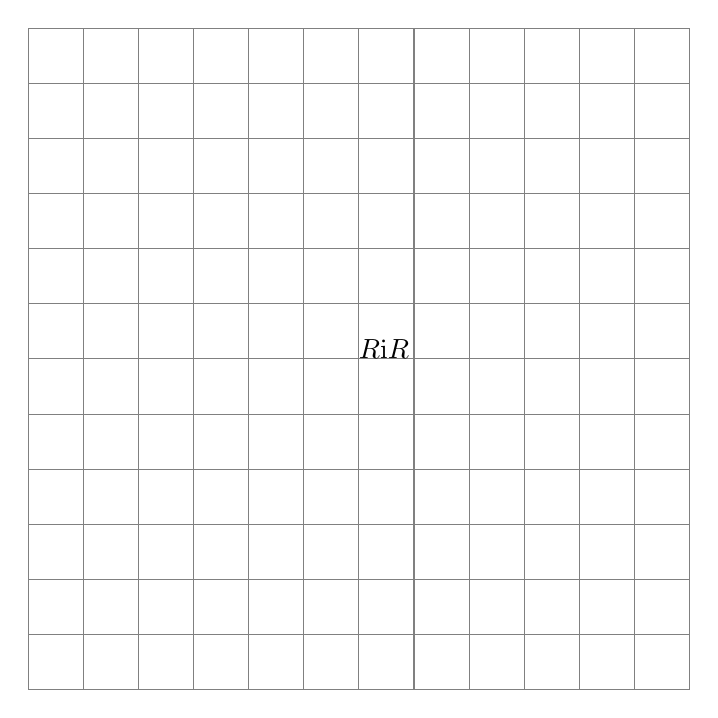
\begin{tikzpicture}[scale=0.7]
  \tkzInit[xmax=6,ymax=6,xmin=-6,ymin=-6]
   \tkzGrid
   \tkzAxeX[label=$\RR$]
   \tkzAxeY[label=$\ii\RR$]
   %\draw[ thick,latex-latex] (-1,4) -- (4,-6) node[anchor=south west] {$a$}; % two points for drawing 2x+y=2
  %\tkzText[above](0,6.75){Desired Output}
\end{tikzpicture}
\end{center}

Aus der letzten Aufgabe kann man sehen, dass die Multiplikation mit komplexen Zahlen Rotationen und Streckungen entspricht, ganz analog wie wir weiter vorne schon gesehen haben, dass $\ii$ der Rotation um $90^{\circ}$ entgegen dem Uhrzeigersinn entspricht.

\subsection{Aufgaben}

\begin{aufgabe}{Potenzen von $\ii$}
  Berechne $\ii^2,\ii^3,\ii^4,\ldots,\ii^9$. Siehst du ein System?
\end{aufgabe}

% \loesung{2cm}

\begin{aufgabe}{Wurzeln von minus Vier}
  Finde alle komplexen Zahlen $x\in\CC$, die $x^2+4=0$ erf\"ullen.

  \emph{Hinweis:} Errate ein paar Kandidaten für~$x$ und rechne einfach die Probe. Wenn du eine Lösung gefunden hast, wirst du eine zweite auch bald entdecken.
\end{aufgabe}
\begin{aufgabe}{Wurzeln von minus Zwei}
  Finde alle komplexen Zahlen $x\in\CC$, die $x^2+2=0$ erf\"ullen.
\end{aufgabe}

% \loesung{2cm}

\begin{aufgabe}{Nochmal Imaginärteil}
  Berechne den Imaginärteil von $\frac{7-2\ii}{5+\ii}$.
\end{aufgabe}

% \loesung{2cm}

\begin{aufgabe}{* Ordnung der komplexen Zahlen}
 Man kann sagen, dass eine relle Zahl größer gleich einer anderen ist, zum Beispiel gilt $3\leq 7$ oder $-4\leq \frac{3}{2}$. Auf der Zahlengerade entspricht dies der Tatsache, dass $7$ weiter rechts liegt als $3$ beziehungsweise $-4$ weiter links liegt als $\frac{3}{2}$. Wir wollen schauen, ob wir das auch auf den komplexen Zahlen sagen können (also "`weiter rechts"' auf der Gaußschen Zahlenebene erklären).
 \begin{enumerate}
   \item Angenommen wir haben eine reelle Zahl $a$ mit $0\leq a$ und wir multiplizieren $a$ mit einer weiteren reellen Zahl $x\geq 0$. Was gilt dann für $a\cdot x$ und $0$? Mache dir das anhand von Beispielen für $a$ und $x$ klar.
   \item Angenommen wir haben eine reelle Zahl $a$ mit $0\leq a$ und wir multiplizieren $a$ mit $x< 0$. Gilt dann $a\cdot x\geq 0$ oder $a\cdot x \leq 0$? Mache dir das anhand von Beispielen für $a$ und $x$ klar.
   \item Kann $\ii \geq 0$ sein? Kann $\ii \leq 0$ sein? \\
	\emph{Hinweis:} Zeige, dass beides nicht gelten kann, wenn die beiden Regeln (a) und (b) immer noch gelten sollen. Also ist sowohl $\ii\geq 0$ als auch $\ii\leq 0$ falsch!
 \end{enumerate}
\end{aufgabe}

% \loesung{3cm}



\end{document}
